\chapter{Conclusions and possible improvements}
\label{chap:ch6}

The main focus of this thesis is classifying images of digital breast tomosynthesis and detecting the tumors present in the cancerous ones. The classification is achieved by passing 22 slices from each 3D scan, resizing it to $512\times512$, through a GoogLeNet model, which returns an array of 2 values between 0 and 1, representing the probability that the image submitted is normal or cancerous. The model is evaluated both in the train phase, by comparing loss graphs, and also in the test phase, by comparing confusion matrices and computing the accuracy, precision and recall.

The detection is performed in a similar way, meaning that the images are sent as 22 individual slices of size $512\times512$. However, the model returns three values: the array of bounding boxes that might have tumors present, an array of integer values representing the classes, benign or malign that these tumors belong to, and an array of values between 0 and 1 representing the probability of the bounding boxes existing. The loss of these predictions is computed directly in the architecture of the model, both for the train and test losses. Because the test evaluation was done in the form of a loss graph, I did not compute the IoU value of these predictions.

In this thesis, I managed to compare results from different experiments conducted on the GoogLeNet classification model. There have been six experiments and out of all of them, the best model found has an accuracy of 0.6232; precision and recall for cancer images are 0.6694 and 0.4922, respectively. The hyper-parameters for this configuration are: learning rate of 0.0001, Adam optimizer, a Step learning rate decay of step 5 and gamma 0.1.

The six experiments on the detection model proved to be more fruitful, achieving an overall better loss for both test and train losses. The final configuration of these experiments achieved a train loss of 0.8469 maximum and 0.02313 minimum, while the train loss was 1.906 maximum and 1.315 minimum. The hyper-parameters include a learning rate of 0.0001, a CosineAnnealingLR learning rate decay with a minimum of $1e^{-6}$ learning rate, called after each batch of size 16 in the dataset.

As for the possible improvements, GoogLeNet proved to not be a worthy architecture for the classification of cancer tumors in digital breast tomosynthesis images because of the low accuracy obtained. I propose a different architecture, maybe DenseNet or ResNet to train and compare the results obtained by GoogLeNet. Additionally, I would increase the length of the dataset even more by including all the slices, keeping in mind the risk that some inputs might overpower others, especially considering the fact that the lowest number of slices an image has in the database is 22, and the highest number is 120.

However, for the EfficientDet model, I am quite happy with the results of the trained model. I would maybe experiment with other types of EfficientDet, from D1 to D5. I do have some concerns, mainly the fact that the test loss seems to slightly increase from epoch to epoch while the train loss decreases. While the CosineAnnealing learning rate decay proved to work well with the model, I would experiment with other types of learning rate decay, such as OneCycle.

\section{SWOT Analysis}

The SWOT analysis presented in the image \ref{fig:fig44} identifies the strengths, weaknesses, opportunities, and threats for my MammoDetect system.

\begin{figure}[H]
    \centering
    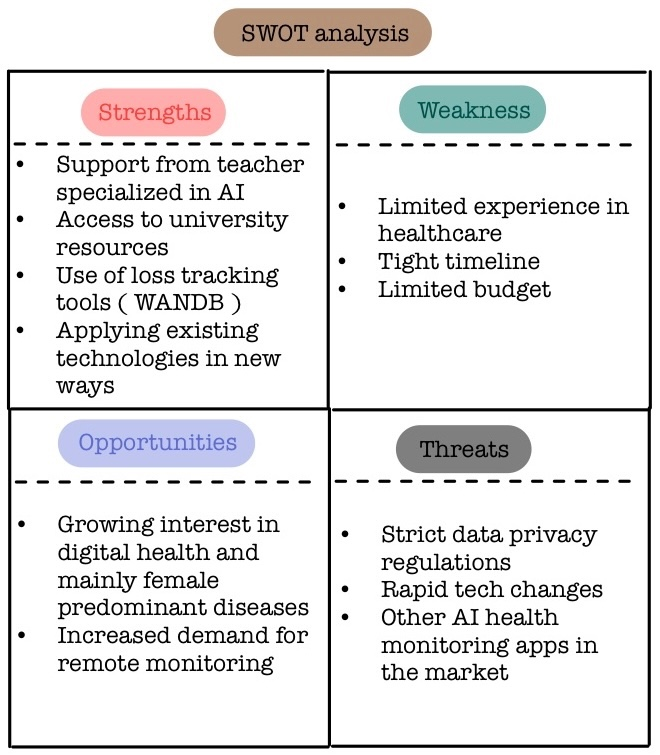
\includegraphics[width=0.5\linewidth]{figures/Figure54.png}
    \caption{SWOT analysis}
    \label{fig:fig44}
\end{figure}

\textbf{Strengths}:
The project benefits from the expertise of a professor in artificial intelligence, providing valuable guidance. I have access to university resources and facilities, such as libraries, as licenses. I used existing technologies but applied them innovatively, which can provide competitive advantages.

\textbf{Weaknesses}:
I have limited experience in the healthcare sector, which can affect my understanding and correct approach to specific problems. The project has a strict deadline, which can create pressure and impact the quality of work. Financial resources are limited, restricting the ability to invest in advanced technologies or necessary equipment.

\textbf{Opportunities}:
There is a growing interest in digital health solutions, especially for diseases that predominantly affect women, offering a target market. There is an increasing demand for remote monitoring solutions, which can create opportunities for the adoption of the technology developed by the project.

\textbf{Threats}:
Strict data protection regulations can create obstacles in the collection and management of patient data. Technology evolves rapidly, which can make the solutions developed quickly outdated. There are already other AI-based tumor detection applications on the market, creating significant competition.
